\documentclass[11pt]{article}
\usepackage[letterpaper,margin=1in]{geometry}
\usepackage[T1]{fontenc}
\usepackage{lmodern,amsmath,amssymb,amsthm,mathtools,booktabs,tabularx,tikz}
\usetikzlibrary{arrows.meta,positioning}
\usepackage{microtype,enumitem,fancyhdr,needspace}
\usepackage[hidelinks]{hyperref}
\setlength{\parindent}{0pt}\setlength{\parskip}{4pt}
\setlist{nosep,leftmargin=*}
\pagestyle{fancy}\fancyhf{}\fancyhead[L]{\small What Makes an Oracle?}\fancyhead[R]{\small Research edition 001v2}\fancyfoot[C]{\thepage}\setlength{\headheight}{14pt}
\newtheorem{theorem}{Theorem}[section]
\newtheorem{definition}[theorem]{Definition}
\newtheorem{corollary}[theorem]{Corollary}
\newtheorem{proposition}[theorem]{Proposition}
\newcommand{\T}{\mathcal T}\newcommand{\K}{\mathcal K}\newcommand{\I}{\mathcal I}\newcommand{\A}{\mathcal A}
\newcommand{\pf}[1]{\unskip\hspace{.6em plus 1fill}\textit{Proof: Appendix A.#1.}}
\begin{document}
\begin{center}
{\LARGE\bfseries What Makes an Oracle?\par}
\vspace{5pt}{\large Minimal Ignorance, Epistemic Topology, and the\par Computational Limits of Recognition\par}
\vspace{15pt}Research Director: Brian Tenneson\\
Joint mathematical development: Picard and DATA MIND\\
AMLD+0 research framework\\[5pt]
\textsc{Research edition 001v2 $\vert$ November 24, 2026}
\end{center}
\begin{abstract}
We propose a property-based, extremal definition of an oracle: an automated theorem prover (ATP) whose mathematical ignorance is minimal. Ignorance is the complement of explicitly certified knowledge in a fixed universe of truths; no numerical measure, special architecture, self-awareness, or privileged answer interface is required. We distinguish minimal from least ignorance and current knowledge from eventual and resource-bounded discovery. For an upward-directed family of attainable knowledge profiles with countable union, the natural positive-information topology is Baire exactly when a greatest profile is attained. In that case the greatest profile is comeager; otherwise the entire profile space is meager in itself. We establish effective realization under uniform certified dovetailing, an obstruction under unrestricted sound extensions of arithmetic knowledge, and finite classes of ordinary ATPs with a unique least-ignorance member that no uniform computable selector can identify. We further separate the complexity of recognition from the complexity of executing an oracle. These results synthesize earlier work on cartographic order, resource-indexed warrant, and noncomputable finality while preserving independent verification. The existence of a nontrivial absolute oracle remains open as a research question until its admissibility and knowledge contract is specified; under one unrestricted effective arithmetic interpretation we prove nonexistence.
\end{abstract}
\vspace{3pt}
\begin{center}\fbox{\parbox{0.87\linewidth}{\centering\large\textbf{An oracle is an ATP whose ignorance is minimal.}\\[5pt]\normalsize An extremal property of a machine, not an instruction for how it must operate.}}\end{center}
\setcounter{tocdepth}{1}
\makeatletter
\renewcommand*\l@section{\@dottedtocline{1}{0em}{2.5em}}
\makeatother
\tableofcontents
\par\bigskip
\section{From what an oracle does to what it is}
The research question is not how to supply a theorem prover with a magical answer service. It is whether an ordinarily programmable ATP can possess an exceptional mathematical property even when the property is not effectively recognizable. The term \emph{oracle} in this paper is a proposed usage and must not be confused with Turing's relative-computability oracle \cite{turing}, an interface granting access to a specified set or function. An extremal ATP need not have such access.

The Research Director's observation is that ignorance can be the objective of the theory even when the machine does not explicitly evaluate that objective. A finite program might attain a mathematical optimum without containing either a description of that optimum or a test for its attainment. This is a question of existence, realization and recognition, not of implementation by declaration.

Three earlier manuscripts motivate the present work. The September 4 Dreamer paper \cite{dreamer}, Sections 3--7, separates resource-bounded warrant and four ideal guidance interfaces from the independent checking of certificates. The September Omnicartographer paper \cite{cart}, Sections 7--8 and Theorem 20.1, develops informational extension and the directed maximum criterion. The October Completion B paper \cite{boundary}, Section 7, shows that a computable process with at most one strict horizon decrease can have an attained final value without a computable uniform last-stage decision. We transfer these ideas to a knowledge-complement objective. The statements and proofs below specify their own hypotheses; none assumes an actual external oracle.

\section{Knowledge and ignorance}
Fix a set $\T$ of true, finitely encoded propositions in a declared semantics, and a nonempty set $\A$ of admissible ATPs. Except for the varying-contract regime in Theorem~\ref{th:arith}, the effective results use a computably coded language, a common decidable certificate checker $V(\varphi,c)$ sound for $\T$, and ordinary finite programs. Soundness means that every accepted conclusion lies in $\T$. Completeness is not presumed. Define
\[
K_V=\{\varphi:\exists c\; V(\varphi,c)=1\}\subseteq\T.
\]
An ATP is modeled by a finite program that emits finitely encoded conclusion--certificate pairs, possibly indefinitely; it has no external oracle access in the effective constructions below. A trusted ledger records accepted conclusions, including any initial certified entries (which may be treated as initial emissions). The ledger is monotone and admission consists exactly of applying the frozen checker to these pairs. Each finite computation stage handles only finitely many pairs; all submitted pairs are eventually checked. Unless specified otherwise, knowledge means the set of distinct conclusions actually admitted in a persistent ledger during a run, rather than all logical consequences implicit in the axioms. For deterministic runs, write $\K_t(A)$ for the conclusions admitted through step $t$, and $\K(A)=\bigcup_{t\in\mathbb N}\K_t(A)$ for eventual knowledge. This is a mathematical profile of the entire run, not an assertion that infinitely many certificates are simultaneously stored at a finite time.

\begin{definition}[Ignorance and oraclehood]\label{def:oracle}
For the fixed contract, let
\[
\I(A)=\T\setminus\K(A).
\]
An \emph{oracle} is an ATP $O\in\A$ with no $B\in\A$ satisfying $\I(B)\subsetneq\I(O)$. A \emph{least-ignorance oracle} satisfies $\I(O)\subseteq\I(B)$ for every $B\in\A$.
\end{definition}
The same definition applies to a different frozen profile, such as $\K_t(A)$, provided it is not changed mid-argument. This is a property-based definition, not an absolute intrinsic property of program code: changing the admissible comparison class can change oraclehood while leaving the code unchanged. Ignorance is not a numerical quantity. Minimality is not leastness. Multiple programs can share an optimal profile; uniqueness of profile does not establish uniqueness of program or identity.

\begin{theorem}[Epistemic duality]\label{th:dual}
For a common universe $\T$, $\K(A)\subseteq\K(B)$ if and only if $\I(B)\subseteq\I(A)$. Hence oracles correspond exactly to maximal attainable knowledge profiles and least-ignorance oracles correspond to greatest attainable profiles.\pf{1}
\end{theorem}

The definition is factive: it does not count mistaken beliefs as knowledge. For a true proposition $\varphi$, ignorance of $\varphi$ means that $\varphi$ is absent from the specified knowledge profile. In classical epistemic notation, ignorance about \emph{whether} a sentence $\psi$ holds is often modeled by $\neg K\psi\land\neg K\neg\psi$. With factivity and a bivalent semantics, ignorance about whether $\psi$ holds reduces to absence of the true one of $\psi$ and $\neg\psi$, provided both alternatives are expressible and the epistemic operator is interpreted by membership in the same certified profile. The present operational ledger is not assumed closed under logical consequence, nor is the absence of a certificate a certificate of nonderivability. This avoids the logical-omniscience idealization noted in \cite{dreamer}.

\begin{center}
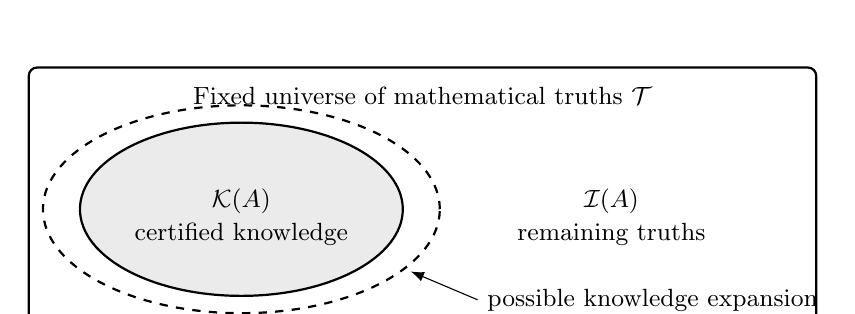
\begin{tikzpicture}[font=\small,>=Latex]
\draw[rounded corners=3pt,thick] (0,0) rectangle (10,3.25);
\node[anchor=north] at (5,3.12) {Fixed universe of mathematical truths $\T$};
\draw[thick,fill=black!8] (2.7,1.45) ellipse (2.05 and 1.1);
\draw[thick,dashed] (2.7,1.45) ellipse (2.52 and 1.32);
\node at (2.7,1.55) {$\K(A)$};\node at (2.7,1.13) {certified knowledge};
\node at (7.4,1.55) {$\I(A)$};\node at (7.4,1.13) {remaining truths};
\draw[->] (5.7,.3) -- (4.85,.66);\node[anchor=west] at (5.7,.3) {possible knowledge expansion};
\end{tikzpicture}

\small Figure 1. Ignorance is the complement; the dashed boundary illustrates possible knowledge growth.
\end{center}

\section{Attainment, incomparability and extension}
Write $X=\{\K(A):A\in\A\}\subseteq\mathcal P(\T)$, ordered by inclusion. The profile family is \emph{directed} when every pair has a common upper bound in $X$. Define
\[
K^*=\bigcup_{K\in X}K,\qquad I^*=\T\setminus K^*=\bigcap_{A\in\A}\I(A).
\]
The set $I^*$ is the infimum of the attainable ignorance sets in the ambient powerset, ordered by inclusion. Whether it is attained by an admissible machine is a separate question.
\begin{theorem}[Order-theoretic existence and obstruction]\label{th:order}
(i) A nonempty finite $X$ has a maximal member. (ii) If every chain in $X$ has an upper bound in $X$, it has a maximal member; if in addition $X$ is directed, it has a greatest member. (iii) $I^*$ is attained exactly when $K^*\in X$. (iv) In a directed family, every maximal member is greatest.\pf{2}
\end{theorem}
Part (ii) is the knowledge-profile version of the Cartographer criterion in \cite[Theorem 20.1]{cart}; it is not a new application of Zorn's lemma in order theory. Its force here is to identify precisely the closure obligations of an oracle construction.

\textbf{Examples.} With $\T=\{p,q,r\}$ and $X=\{\{p\},\{q\}\}$, both profiles are maximal, neither is greatest, and both have nonempty ignorance. With $\T=\{q_0,q_1,\ldots\}$ and $X=\{\{q_0,\ldots,q_{n-1}\}:n\in\mathbb N\}$, there is no maximal member even though the ambient infimum of ignorance is empty. These are realizable by restricted certificate-output programs for elementary tautologies. Restricting the class is essential; the examples do not demonstrate exceptional intelligence.

\section{Epistemic topology and the Baire criterion}
A topology can be derived from finite positive observations of knowledge instead of prescribing topological smallness as an oracle axiom. For $\varphi\in\T$ put
\[
U_\varphi=\{K\in X:\varphi\in K\},\qquad U_F=\{K\in X:F\subseteq K\}
\]
for finite $F\subseteq\T$. The sets $U_F$ are a basis for the positive-information topology $\tau_+$ on $X$. They encode finite witnessed assertions of membership. The topology is $T_0$, since distinct profiles differ on some proposition, but is not generally Hausdorff: if $K\subsetneq L$, every open neighborhood of $K$ also contains $L$.

A set is nowhere dense if its closure has empty interior; a meager set is a countable union of nowhere dense sets. A space is Baire if every countable intersection of dense open subsets is dense. We use these standard definitions without assuming a metric.
\begin{theorem}[Baire--oracle equivalence]\label{th:baire}
Let $X$ be nonempty and directed, and let $K^*$ be countable. The following are equivalent:
\begin{enumerate}[label=(\roman*)]
\item $X$ with $\tau_+$ is Baire;
\item $X$ is not meager in itself;
\item $K^*\in X$ (equivalently, a least-ignorance oracle exists).
\end{enumerate}
When these hold, the singleton $\{K^*\}$ is dense and comeager, and the other profiles form a meager set. If they fail, $X$ is meager in itself and has no oracle.\pf{3}
\end{theorem}
\begin{center}
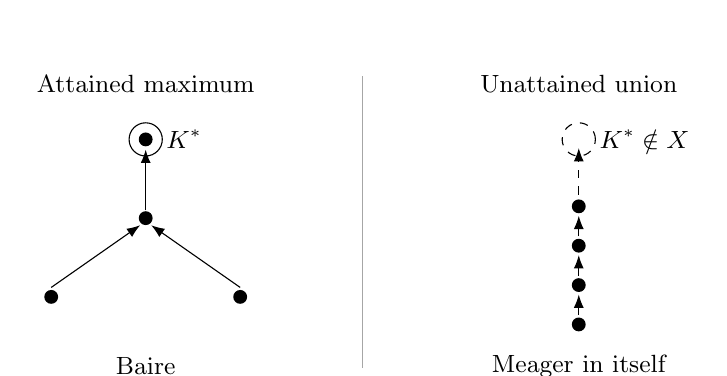
\begin{tikzpicture}[font=\small,>=Latex,x=1cm,y=1cm]
\node at (2.5,3.7) {Attained maximum};\node at (8,3.7) {Unattained union};
\foreach \x/\y in {1.3/1,3.7/1,2.5/2,2.5/3} {\fill (\x,\y) circle (2.5pt);}
\draw[->] (1.3,1.12)--(2.43,1.91);\draw[->] (3.7,1.12)--(2.57,1.91);\draw[->] (2.5,2.1)--(2.5,2.87);
\draw (2.5,3) circle (6pt);\node[right] at (2.64,3) {$K^*$};
\foreach \y in {.65,1.15,1.65,2.15} {\fill (8,\y) circle (2.5pt);}
\foreach \y in {.77,1.27,1.77} {\draw[->] (8,\y)--(8,\y+.26);}
\draw[dashed,->] (8,2.3)--(8,2.89);\draw[dashed] (8,3) circle (6pt);\node[right] at (8.14,3) {$K^*\notin X$};
\node at (2.5,.12) {Baire};\node at (8,.12) {Meager in itself};
\draw[black!35] (5.25,.1)--(5.25,3.8);
\end{tikzpicture}

\small Figure 2. Two illustrative directed knowledge orders. Arrows indicate inclusion, not executable transitions.
\end{center}
This is a theorem about the space of attainable \emph{profiles}, not a theorem that $\I(O)$ itself is meager in the space of propositions. On a discrete truth universe the only meager set is empty. A topology appropriate for literal ignorance would need separate mathematical motivation. Moreover, comeagerness in $\tau_+$ is not a frequency or probability statement about program implementations.

\Needspace{5\baselineskip}
\begin{theorem}[A compactness realization criterion]\label{th:compact}
If $X\subseteq\{0,1\}^{\T}$, identified via characteristic functions, is nonempty, directed and closed in the product topology, then $K^*\in X$. As an abstract powerset theorem this holds even for uncountable $\T$ in ZFC; that generalization is outside the finitely encoded ATP model of Section 2.\pf{4}
\end{theorem}
The positive topology and the product topology have different evidentiary meanings: the latter also observes negative membership. Product closure is a substantive assumption. For finite initial segments of an infinite set the product closure contains their union, but the original class does not. Adding a limit profile without an admissible realizing ATP does not solve the oracle construction problem.

\section{When an oracle can be coded}
\begin{theorem}[Uniform certified amalgamation]\label{th:amalg}
Suppose $\A$ is given by a nonempty, finite or computably enumerable list of codes of ordinary ATPs, all run under the same decidable sound checker, with knowledge defined by eventual accepted outputs. If the class admits the machine that fairly dovetails these runs and retains their accepted outputs, it has a least-ignorance oracle.\pf{5}
\end{theorem}
This supplies a real algorithm under its hypotheses: enumerate codes, interleave finite simulation steps, check outputs, and retain accepted certificates. It may incur greater time and storage costs than a specialist on a particular task. The theorem concerns eventual coverage, not efficiency, architectural identity, or any fixed budget. Closure under pairwise amalgamation alone does not give effective countable amalgamation; a list of codes may not be effectively obtainable or its dovetailer admissible.

\begin{corollary}[The fixed-verifier ceiling]\label{th:ceiling}
If an unrestricted effective class permits a universal certificate enumerator for its fixed checker $V$, then that machine attains least ignorance $\T\setminus K_V$.\pf{6}
\end{corollary}
This result forces an important refinement of the research program. For a sound recursively axiomatized arithmetic theory, a brute-force proof enumerator is already a least-ignorance oracle under unrestricted eventual theorem coverage relative to that fixed verifier. It need not solve a single difficult benchmark quickly. The definition is simple, but whether it identifies an exceptional ATP depends on the chosen knowledge contract. This is a limitation of eventual coverage as a model of intelligence, not a reason to conceal the theorem.

\begin{theorem}[Unrestricted sound-extension obstruction]\label{th:arith}
Let $\T$ be the true sentences of first-order arithmetic in the standard natural numbers. Suppose each admissible ATP has computably enumerable sound eventual knowledge, and for every $A\in\A$ and every $\varphi\in\T\setminus\K(A)$ there is an admissible $B$ with $\K(A)\cup\{\varphi\}\subseteq\K(B)$. Then no oracle exists.\pf{7}
\end{theorem}
The extension assumption is semantic and nonuniform. It may allow adding a true sentence as an axiom, hence changing the proof contract. It cannot hold for any fixed sound decidable checker on the full arithmetic truth domain: $K_V$ is computably enumerable and therefore omits a truth, which no admissible output under that checker could add. The extension hypothesis provides no effective method for recognizing a safe extension. Theorem~\ref{th:arith} and Corollary~\ref{th:ceiling} therefore concern different regimes, not contradictory conclusions. For example, the class of all computably enumerable subsets of arithmetic truth satisfies the extension hypothesis, as adjoining one fixed true sentence to any such set preserves computable enumerability and soundness. This is a semantically specified class of output profiles, not a computably enumerable list of uniformly sound verifiers or an effective test of soundness.

\section{The oracle that exists but cannot uniformly be found}
The central question is whether computability of an ATP's operation implies computability of identifying an optimal ATP. It does not. Let $H$ be the halting set for machines run on blank input; use the convention that no halt is recorded at step zero. In the examples below all propositions are simple, distinct true arithmetic sentences with known finite certificates, and all outputs pass a common sound checker. Delaying an output is a permissible program behavior.
\begin{theorem}[Computationally elusive oracle selection]\label{th:select}
There exists a uniformly computable family of two-element classes of ordinary ATPs with a fixed finite truth domain, each containing a unique least-ignorance ATP, such that no total computable selector chooses that ATP from every pair. For this family a halting oracle suffices, and any uniform correct selector (returning the selected index in the ordered pair) computes $H$.\pf{8}
\end{theorem}
Let $\T=\{p,q,r\}$. Machine $A$ emits the fixed certified pair for $p$; machine $B_e$ emits nothing until it detects that program $e$ halts, then emits the fixed certified pairs for $p$ and $q$. No machine emits $r$. Their eventual profiles are as follows:
\begin{center}
\begin{tabular}{llll}\toprule
Condition & $\I(A)$ & $\I(B_e)$ & Least ignorance attained by\\\midrule
$e$ halts & $\{q,r\}$ & $\{r\}$ & $B_e$\\
$e$ never halts & $\{q,r\}$ & $\{p,q,r\}$ & $A$\\\bottomrule
\end{tabular}
\end{center}
The least ignorance set is nonempty in both cases. No external oracle is needed to run either candidate. In contrast, a classical halting oracle would resolve the uniform selection problem. The distinction between the extremal and the Turing sense of oracle is now a theorem in a common restricted model.

\begin{theorem}[Finite attainment without a computable stopping rule]\label{th:stop}
There is a uniformly computable family of persistent knowledge runs whose ignorance decreases at most once, whose minimum is attained at a finite stage in every run, and for which no total computable procedure returns a valid stabilization stage for all runs. For the exhibited family, the uniform finality predicate has Turing degree $0'$.\pf{9}
\end{theorem}
This is the direct knowledge-set analogue of \cite[Theorem 7.3]{boundary}. The construction distinguishes a machine attaining its minimum along its own trajectory from a machine being optimal among all admissible architectures. The first alone does not imply the second; the trajectory may omit better admissible profiles. If the comparison is restricted to its own stages, the stabilized profile is greatest in that restricted family.

\begin{center}
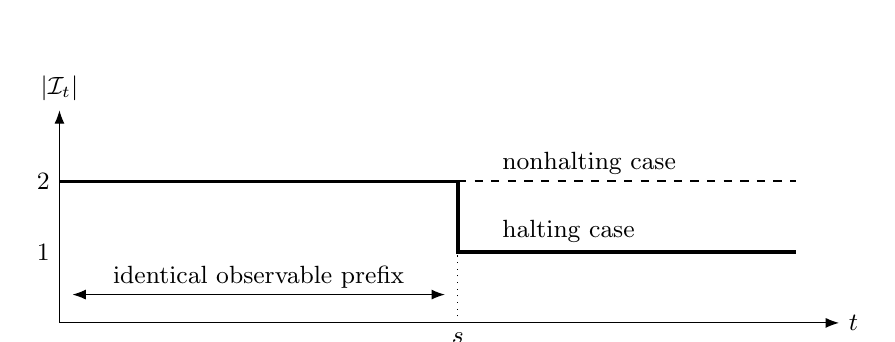
\begin{tikzpicture}[>=Latex,font=\small,x=1.1cm,y=.9cm]
\draw[->] (0,0)--(9,0) node[right] {$t$};\draw[->] (0,0)--(0,3) node[above] {$|\I_t|$};
\node[left] at (0,2) {2};\node[left] at (0,1) {1};
\draw[thick,dashed] (0,2)--(8.5,2);\draw[very thick] (0,2)--(4.6,2)--(4.6,1)--(8.5,1);
\draw[dotted] (4.6,0)--(4.6,2);\node[below] at (4.6,0) {$s$};
\node[anchor=west] at (5,2.25) {nonhalting case};\node[anchor=west] at (5,1.3) {halting case};
\draw[<->] (.15,.4)--(4.45,.4);\node at (2.3,.65) {identical observable prefix};
\end{tikzpicture}

\small Figure 3. A finite minimum can already have been attained without a general test for finality.
\end{center}
\begin{theorem}[General finite-class recognition boundary]\label{th:recognize}
For arbitrary finite nonempty lists of effective certificate enumerators, deciding whether a designated member is maximal in eventual knowledge is computable in $0''$. For a fixed sound decidable checker admitting a computable infinite sequence of distinct certified truths, there is a uniform family of two-element lists for which the recognition predicate is $\Sigma^0_2$-complete (and thus has Turing degree $0''$).\pf{10}
\end{theorem}
Unlike Theorem~\ref{th:select}, the hardness family for Theorem~\ref{th:recognize} need not be directed or have a unique greatest profile. This distinction matters: selection under a promise and recognition without that promise are different decision problems. We make no claim that every fixed family has a hard recognition problem, or that every oracle fails to know its status. An individual oracle may have a simple proof of its optimality.

\begin{proposition}[Finite observations do not certify optimality]\label{th:finiteobs}
There is no uniformly correct terminating observation procedure that decides oraclehood from the accepted-output prefixes of a designated ATP and its competitor, even for the promised pairs of Theorem~\ref{th:select}. Observations may include silence for a finite number of simulated steps, but exclude program codes, internal states and any oracle for future behavior.\pf{12}
\end{proposition}
This is a statement about observation, not a claim that a proof inspecting source code is always impossible. It concerns a uniformly correct terminating test of the specified kind.

\section{Knowledge versus the capacity to discover}
The original four-interface framework \cite{dreamer} suggests distinguishing knowledge of truths about settlement roles, resource allocation, strategies and certificates. We can encode such claims in disjoint tagged truth domains $\T_j$ with appropriately sound certificate policies. Then, with $\K_j(A)=\K(A)\cap\T_j$,
\[
\T=\bigsqcup_{j=1}^m\T_j,\qquad \I_j(A)=\T_j\setminus\K_j(A).
\]
\begin{proposition}[Joint versus componentwise minimality]\label{th:category}
With disjoint tags, the global knowledge inclusion order is the componentwise order. An ATP minimizing ignorance in every component is globally minimal. Global minimality need not imply minimality in any individual component.\pf{11}
\end{proposition}
For example, two specialists can outperform a generalist separately while each loses knowledge in the other domain. This is a mathematical reason to allow categories without declaring a category of ignorance to be topologically meager. The four historical interfaces are not automatically independent axes and their ideal answers need their own semantics and warrants.

The resource-indexed refinement is to use a common task or workload contract and define $\K_{\le b}(A)$ as the set of truths with a valid output obtainable by cost $b$ in the specified experiment. For independent per-query experiments, state reset, inputs and information must be shared; for a single ledger run, include scheduling and all other charged work. Define the tagged profile
\[
\widehat K(A)=\{(\varphi,b):\varphi\in\K_{\le b}(A)\},\qquad b\in\mathbb N.
\]
Order and topology results apply to the common label universe $\T\times\mathbb N$ when their respective hypotheses hold. Here the labels encode budget-indexed attainability, not additional mathematical propositions asserted true by the machine. The cost contract must fix whether attainability means a deterministic run or some explicitly quantified set of legal runs; no comparison mixes these conventions. The amalgamation theorem does not automatically apply: a combined program can lose early-budget knowledge through simulation overhead. Eventual coverage equality can coexist with arbitrarily different finite-time discovery costs. One must not claim a speed advantage without a fair fully charged comparison.

\section{Consequences and open research}
\begin{tabularx}{\linewidth}{@{}p{.34\linewidth}X@{}}\toprule
Question & Mathematical status in this paper\\\midrule
Is an oracle defined by its architecture? & No architectural requirement in Definition~\ref{def:oracle}.\\
Must it use a Turing oracle? & No: Theorems~\ref{th:amalg} and \ref{th:select} give effective instances.\\
Is minimum ignorance always attained? & No: Theorem~\ref{th:order} and the infinite-chain example; Theorem~\ref{th:arith} under its extension contract.\\
Can topology characterize attainment? & Yes, under the precise hypotheses of Theorems~\ref{th:baire} and \ref{th:compact}.\\
Can computation uniformly identify an oracle? & Not in general: Theorems~\ref{th:select}--\ref{th:recognize}.\\
Is an oracle's literal ignorance meager? & Not proved; a distinct truth-space topology and hypotheses are needed.\\
Is an oracle necessarily fast or self-aware? & Neither follows from the definition.\\\bottomrule
\end{tabularx}

We propose three open directions. First, find naturally motivated admissible classes of ATPs whose resource-indexed knowledge profiles have genuine, nontrivial attained minima. Second, identify structural conditions on theorem spaces under which residual ignorance is topologically small, without making smallness part of the definition. Third, characterize what evidence a machine can obtain about its own extremal position when the property is not uniformly decidable. These questions concern oracle theory itself; no GBG+S or gift mechanism is needed for the stated theorems. A separate investigation may later ask whether an authorized transformation can realize an oracle while preserving certification and identity.

The principal conceptual result is that an oracle can be defined by what it is. The principal mathematical result is a separation: an optimum can be attained by an ordinary finite program even though its uniform identification is not an ordinary computable task. The central challenge is now to find a meaningful epistemic contract in which the optimum represents mathematical discovery ability rather than mere unbounded enumeration.

\appendix
\section{PROOFS}
All results use ordinary classical mathematics; the product compactness result uses ZFC. For effective arguments a finite code is simulated in discrete steps; its output is admitted only by the declared checker. Proofs are collected here so that the main text states the research results without conflating them with empirical claims.

\subsection{Proof of Theorem~\ref{th:dual}: epistemic duality}\label{proof:dual}
For $K,L\subseteq\T$, if $K\subseteq L$ and $x\in\T\setminus L$, then $x\notin K$, so $x\in\T\setminus K$. Conversely, apply the same implication to the complements and use double complementation relative to $\T$. Strict inclusion is reversed as well. The definitions of maximal/minimal and greatest/least now yield the claims.\hfill$\square$

\subsection{Proof of Theorem~\ref{th:order}: order-theoretic existence}
(i) A strictly increasing sequence in a finite partially ordered set cannot repeat and must stop after finitely many steps; any nonmaximal terminal point would permit another step. (ii) The chain hypothesis and Zorn's lemma supply a maximal $M$. For any $K\in X$, directedness gives $L\in X$ containing $M\cup K$. Maximality forces $L=M$, hence $K\subseteq M$. (iii) By definition every $K$ is contained in $K^*$. If a greatest member $M$ exists it contains their union, while $M\subseteq K^*$, hence equals $K^*$. Conversely if $K^*\in X$ it is greatest. Duality gives the claim for $I^*$. (iv) The directedness argument in (ii) uses only maximality, not Zorn's lemma.\hfill$\square$

\subsection{Proof of Theorem~\ref{th:baire}: Baire--oracle equivalence}
Each $U_\varphi$ for $\varphi\in K^*$ is nonempty and open. If $U_F$ is a nonempty basic open set, take $K\in U_F$ and $L\in U_\varphi$. A common extension $M\in X$ contains $F$ and $\varphi$, so $U_F\cap U_\varphi\ne\varnothing$. Thus $U_\varphi$ is dense; $X\setminus U_\varphi$ is closed nowhere dense. By countability,
\[
\bigcap_{\varphi\in K^*} U_\varphi=\begin{cases}\{K^*\},&K^*\in X,\\\varnothing,&K^*\notin X.\end{cases}
\]
If $X$ is Baire the intersection is dense and, because $X$ is nonempty, nonempty. If $K^*\notin X$, the complement expression $X=\bigcup_{\varphi\in K^*}(X\setminus U_\varphi)$ shows meagerness in itself. If $K^*\in X$, all nonempty opens contain $K^*$, so every dense open contains it, and every intersection of dense opens is dense. Furthermore every nowhere dense subset omits $K^*$: a subset containing $K^*$ has closure $X$. Hence $X$ is not meager in itself. The countable complement expression establishes comeagerness of $\{K^*\}$. The argument also covers $K^*=\varnothing$: then $X=\{\varnothing\}$. If no greatest element exists, directedness and Theorem~\ref{th:order}(iv) exclude all maximal elements.\hfill$\square$

\subsection{Proof of Theorem~\ref{th:compact}: compactness}
By Tychonoff's theorem the product of copies of the finite discrete compact space $\{0,1\}$ is compact. Its closed subspace $X$ is compact. Each $U_\varphi$ is closed in this product subspace. A finite family of such sets with labels in $K^*$ has nonempty intersection: choose witnesses to each label and use directedness finitely many times. By the finite intersection property their entire intersection is nonempty. Its only possible member is $K^*$, so $K^*\in X$. For the empty family use nonemptiness.\hfill$\square$

\subsection{Proof of Theorem~\ref{th:amalg}: effective amalgamation}
At stage $s$, advance the code enumerator for one step, then advance each simulation whose code has appeared by one step; duplicates can be ignored or treated as distinct simulations. Each enumerated code is eventually simulated and receives arbitrarily many steps. Queue all output certificates and interleave checking so that every output is eventually processed. The common per-pair admission policy and retention ensure the combined accepted knowledge is exactly the union of the input runs' accepted knowledge: inclusion in the union follows because the only outputs are copied from simulated runs and checked under the same frozen policy, and the reverse inclusion follows by fairness. The combined code is finite and belongs to $\A$ by the explicit closure assumption, giving attainment by Theorem~\ref{th:order}. In the finite case the list itself can be hardwired. No decision about eventual nonoutput is needed.\hfill$\square$

\subsection{Proof of Corollary~\ref{th:ceiling}: fixed verifier}
Enumerate all syntactically valid pairs $(\varphi,c)$ and test the total decidable predicate $V$. Emit every accepted pair. Every $\varphi\in K_V$ has some finite witness and is eventually emitted. The acceptance definition precludes admitted conclusions outside $K_V$. Thus $K_V$ is attained, and all other admissible profiles lie inside it.\hfill$\square$

\subsection{Proof of Theorem~\ref{th:arith}: sound extensions}
The set of true first-order arithmetic sentences is not computably enumerable. For completeness, if it were, one could decide truth of each sentence by waiting until either it or its negation appeared. Exactly one must appear in classical standard arithmetic. This would decide the halting problem, since for each machine code one can effectively express the assertion that a finite halting computation exists as an arithmetic sentence (via finite computation coding). Hence no computably enumerable sound profile equals $\T$. For each $A$ choose $\varphi\in\T\setminus\K(A)$; the extension hypothesis supplies $B$ strictly containing $\K(A)$. By duality it has strictly smaller ignorance. No $A$ is minimal.\hfill$\square$

\subsection{Proof of Theorem~\ref{th:select}: elusive selection}
Use the explicit pair $A,B_e$ in Section 6. The three truths and certificates are fixed in advance, and the code of $B_e$ is computably obtained by inserting $e$ into a simulator-and-output program. The profiles in the table follow from the run semantics. In either case strict inclusion holds in one direction, so the least-ignorance program is unique within the pair. A total selector returns index $B_e$ exactly if $e\in H$. Therefore such a selector computes $H$, and is not computable. Given $H$, select according to its bit; thus the family-specific selection problem is exactly of halting degree. The third truth is never emitted in either run. All outputs are sound regardless of the unknown bit.\hfill$\square$

\subsection{Proof of Theorem~\ref{th:stop}: noncomputable stabilization}
Take $\T=\{p,q,r\}$ and initialize the ledger with $p$. Here $t$ is the index of a finite observation stage, not an assertion about the total runtime cost of computing that stage. At stage $t$, use bounded simulation of $e$ for $t$ steps. Include $q$ if a halt has occurred and never add $r$. The finite ledger is uniformly computable, monotone, and changes at most once. If $e$ halts at $s$, its minimum along the run is attained at $s$; otherwise it is attained at zero. Let $F(e,N)$ assert that $\I_t=\I_N$ for all $t\ge N$. A computable search for a later differing set halts exactly if $F(e,N)$ fails, so $H$ decides $F$. At $N=0$, $F(e,0)$ holds exactly when $e$ never halts; hence $F$ computes $H$. If a total computable stage selector existed, simulate $e$ for the selected number of steps. A halt must be recorded there if one ever occurs, since no change may occur later; this decides $H$. Contradiction.\hfill$\square$

\subsection{Proof of Theorem~\ref{th:recognize}: recognition complexity}
For effective enumerators $A,B$, define the computable predicate $E_A(x,s)$ to mean that label $x$ has been emitted and accepted by stage $s$ (with bounded simulation including checking time). Inclusion is equivalent to
\[
\forall x\,\forall s\,\exists t\;[\neg E_A(x,s)\lor E_B(x,t)],
\]
a $\Pi^0_2$ predicate. Thus $0''$ decides inclusion, strict inclusion and, by finitely many comparisons, whether a designated index is maximal. For hardness, let $W_e$ be the standard uniformly enumerated c.e. sets and use the standard $\Sigma^0_2$-complete index set $\mathrm{FIN}=\{e:W_e\text{ is finite}\}$ \cite{soare}. For clarity, membership in FIN is $\exists n\,\forall s\,(|W_{e,s}|\le n)$ for finite stage approximations. To see hardness, given a predicate $\exists u\,\forall v\,R(e,u,v)$ with decidable $R$, at stage $s$ let $m_s$ be the least $u\le s$ satisfying $R(e,u,v)$ for all $v\le s$, or $s+1$ if none exists. Enumerate a fresh number whenever $m_s$ changes (and one at the first stage). If a witness exists, $m_s$ eventually equals the least witness; if none exists, $m_s$ eventually exceeds each fixed bound. The enumerated set is therefore finite exactly when the predicate holds. The uniform program construction gives a many-one reduction to FIN. Use the assumed computable sequence of distinct certified truths $r,q_0,q_1,\ldots$ with computable certificates (for example, distinct syntactic tautologies under a suitable fixed checker). Let $A$ enumerate every $q_n$ and omit $r$. Let $B_e$ enumerate $r$ immediately and enumerate $q_0,\ldots,q_{k-1}$ when $k$ distinct elements of $W_e$ have appeared. If $W_e$ is infinite, $B_e$ strictly dominates $A$. If $W_e$ is finite, $B_e$ lacks some $q_n$ and $A$ lacks $r$, hence they are incomparable. Therefore $A$ is maximal in this two-element class exactly on $\mathrm{FIN}$. The map to the pair is computable, proving the stated $\Sigma^0_2$-complete restriction and the degree bound. We do not assert that the unrestricted recognition predicate is itself $\Sigma^0_2$.\hfill$\square$

\subsection{Proof of Proposition~\ref{th:category}: typed domains}
Inclusion of tagged unions is equivalent to inclusion in each component. If a machine minimizes each component, any global strict improvement would have to strictly improve at least one component, which is impossible. For the converse take two disjoint component domains, each with two truths. Use three admissible knowledge profiles with component sizes $(1,1),(2,0),(0,2)$, where the one-element sets are contained in the corresponding two-element sets. Each profile is incomparable with the others under componentwise inclusion. The first is globally maximal but neither component is maximal among attainable component profiles. Complementation transfers this to ignorance.\hfill$\square$

\subsection{Proof of Proposition~\ref{th:finiteobs}: finite observation}
In the construction of Theorem~\ref{th:select}, choose a nonhalting simulation that produces no accepted output. The designated machine $A$ is then the unique oracle. Any terminating transcript-only rule must decide after some finite observations of both machines. Choose instead an index of a program that halts only after more simulation steps than were observed; the corresponding competitor $B_e$ in the same promised family stays silent through the entire observed prefix and subsequently emits $p,q$. The observer is not given the index $e$ or source code. On equal observed prefixes its adaptive observation choices also agree, so the alternative run reaches the same decision. This has the same finite observed output transcript under the same observation schedule, but $A$ is no longer an oracle. Thus the rule errs on one of the promised pairs. This proof does not require the source codes to coincide; those are not among the permitted observations.\hfill$\square$

\section*{Research provenance and evidence status}
\addcontentsline{toc}{section}{Research provenance and evidence status}
The Research Director proposed ignorance as the objective, its complement-of-knowledge representation, the possibility of attained but computationally elusive minima, and the requirement that topological properties be derived rather than declared. Picard and DATA MIND are conversational research roles used for mathematical development; AMLD+0 describes the research protocol. Edition 001v2 contains a conversational ATLAS audit of the theorem statements, proofs and scope contracts, followed by repair and re-review. It preserves the oracle definition and all twelve mathematical results. The paper contains internally reviewed arguments, not independently machine-checked certificates or peer review. The source attributions are retained from edition 001; the present audit checks the self-contained arguments, not the full contents of the three earlier linked manuscripts. The mathematical results use standard order theory, topology and computability; no exhaustive originality search has been performed. No external agents, paid computations, repository changes or actual oracle implementations are claimed.

\begin{thebibliography}{9}
\bibitem{dreamer} B. Tenneson. \emph{Dreamer and Four-Oracle Extension to DATA MIND 3.2}. September 4, 2026, Sections 3--7. \href{https://btenneson.github.io/pub/cs.LO_Logic_in_Computer_Science/dreamer_four_oracle_data_mind_3_2/}{Publication and PDF}.
\bibitem{cart} B. Tenneson. \emph{Oracle and Omnicartographer Theory: A Running Mathematical Development}. Research edition 003, September 2026, Sections 7--8 and Theorem 20.1. \href{https://btenneson.github.io/pub/cs.LO_Logic_in_Computer_Science/oracle_omnicartographer_theory_003/}{Publication and PDF}.
\bibitem{boundary} B. Tenneson. \emph{Oracle-Attested Mathematical Knowledge: Completion B, An Epistemic Boundary Theorem for Deactivated Sources and Blind Transmission}. Version 1.1, October 30, 2026, Section 7. \href{https://btenneson.github.io/pub/cs.LO_Logic_in_Computer_Science/oracle_attested_mathematical_knowledge_fdwc_b_epistemic_boundary_theorem_1_1/}{Publication and PDF}.
\bibitem{turing} A. M. Turing. Systems of logic based on ordinals. \emph{Proceedings of the London Mathematical Society}, s2-45 (1939), 161--228.
\bibitem{soare} R. I. Soare. \emph{Recursively Enumerable Sets and Degrees}. Springer, 1987.
\end{thebibliography}
\end{document}
